\begin{pastexam}[label={px:ncku-110-prog-05}]{成大資訊聯招 110 學年度 第 5 題}
（計算）

(10\%) Please show the cost of the minimum cost spanning tree for the following graph.
\begin{center}
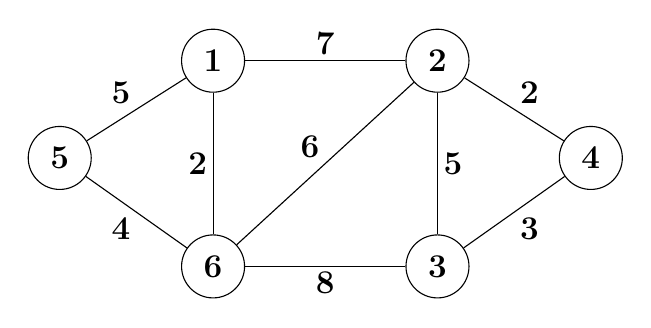
\begin{tikzpicture}[x=0.95cm,y=0.95cm,
  v/.style={circle,draw,minimum size=8mm,inner sep=0pt,font=\bfseries\large},lab/.style={font=\bfseries\large,inner sep=2pt}]
\node[v] (5) at (0.75,-2.3) {5}; \node[v] (1) at (2.8,-1.0) {1}; \node[v] (6) at (2.8,-3.75) {6};
\node[v] (2) at (5.8,-1.0) {2}; \node[v] (3) at (5.8,-3.75) {3}; \node[v] (4) at (7.85,-2.3) {4};
\draw (5) -- node[lab,above left] {5} (1);
\draw (5) -- node[lab,below left] {4} (6);
\draw (1) -- node[lab,left] {2} (6);
\draw (1) -- node[lab,above] {7} (2);
\draw (6) -- node[lab,above left] {6} (2);
\draw (6) -- node[lab,below] {8} (3);
\draw (2) -- node[lab,right] {5} (3);
\draw (2) -- node[lab,above right] {2} (4);
\draw (3) -- node[lab,below right] {3} (4);
\end{tikzpicture}
\end{center}
\end{pastexam}

\begin{pastsoln}
答案：最小生成樹的成本是 $17$，邊是 $(1,6)$、$(2,4)$、$(3,4)$、$(5,6)$、$(6,2)$。

圖有 $6$ 個頂點、$9$ 條邊。 用 Kruskal 演算法（資結書第~24.2~節），邊依權重由小到大看，兩端
已經相連就跳過。 權重相同的邊誰先看都可以，結果的總成本一樣（資結書第~24.1.7~節）。
\begin{center}
\begin{tabular}{clll}
\toprule
權重 & 邊 & 動作 & 之後的元件（兩個頂點以上的） \\
\midrule
2 & $(1,6)$ & 加入 & $\{1, 6\}$ \\
2 & $(2,4)$ & 加入 & $\{1, 6\}$、$\{2, 4\}$ \\
3 & $(3,4)$ & 加入 & $\{1, 6\}$、$\{2, 3, 4\}$ \\
4 & $(5,6)$ & 加入 & $\{1, 5, 6\}$、$\{2, 3, 4\}$ \\
5 & $(5,1)$ & 跳過（$5$、$1$ 已相連） & \\
5 & $(2,3)$ & 跳過（$2$、$3$ 已相連） & \\
6 & $(6,2)$ & 加入，兩個元件合併 & $\{1, 2, 3, 4, 5, 6\}$ \\
\bottomrule
\end{tabular}
\end{center}
加到第 $5 = 6 - 1$ 條邊就連成一棵樹，$(1,2) = 7$、$(6,3) = 8$ 不必再看。 成本
\[
2 + 2 + 3 + 4 + 6 = 17.
\]

\begin{center}
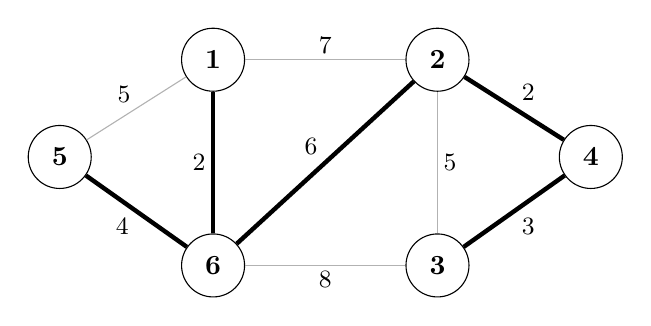
\begin{tikzpicture}[x=0.95cm,y=0.95cm,
  v/.style={circle,draw,minimum size=8mm,inner sep=0pt,font=\bfseries},lab/.style={font=\small,inner sep=2pt}]
\node[v] (5) at (0.75,-2.3) {5}; \node[v] (1) at (2.8,-1.0) {1}; \node[v] (6) at (2.8,-3.75) {6};
\node[v] (2) at (5.8,-1.0) {2}; \node[v] (3) at (5.8,-3.75) {3}; \node[v] (4) at (7.85,-2.3) {4};
\draw[black!30] (5) -- node[lab,above left,text=black] {5} (1);
\draw[black!30] (1) -- node[lab,above,text=black] {7} (2);
\draw[black!30] (6) -- node[lab,below,text=black] {8} (3);
\draw[black!30] (2) -- node[lab,right,text=black] {5} (3);
\draw[line width=1.6pt] (5) -- node[lab,below left] {4} (6);
\draw[line width=1.6pt] (1) -- node[lab,left] {2} (6);
\draw[line width=1.6pt] (6) -- node[lab,above left] {6} (2);
\draw[line width=1.6pt] (2) -- node[lab,above right] {2} (4);
\draw[line width=1.6pt] (3) -- node[lab,below right] {3} (4);
\end{tikzpicture}
\end{center}

\textbf{為什麼一定要用 $(6,2)$}：跳過兩條權重 $5$ 的邊之後，$\{1, 5, 6\}$ 和 $\{2, 3, 4\}$ 之間的
邊只剩 $(6,2) = 6$、$(1,2) = 7$、$(6,3) = 8$，由切割性質（資結書定理~24.1），跨過這個切割最輕的
$(6,2)$ 一定在某棵最小生成樹裡。 用 Prim 從頂點 $1$ 開始也一樣：依序加入 $(1,6) = 2$、
$(6,5) = 4$、$(6,2) = 6$、$(2,4) = 2$、$(4,3) = 3$，總和 $17$。
\end{pastsoln}
